\section{Analisi}

L'analisi del progetto è un'attività cruciale nello sviluppo di qualsiasi sistema \textit{software}. Essa fornisce le 
fondamenta su cui si basa l'intero processo di sviluppo, definendo chiaramente i requisiti e le aspettative 
del sistema. Questa fase non è un processo statico, ma un'attività dinamica che evolve e si raffina continuamente durante 
l'intero ciclo di vita del progetto.\\
È fondamentale sottolineare che l'analisi non si conclude con l'inizio dell'attività di codifica. Al contrario, 
è un processo iterativo che viene costantemente raffinato man mano che emergono nuove informazioni o si incontrano sfide 
impreviste durante lo sviluppo. Questo approccio permette di adattarsi alle mutevoli esigenze del progetto e 
garantisce che il prodotto finale soddisfi le aspettative del cliente.

\subsection{Casi d'uso}

Un'attività fondamentale durante l'analisi del progetto è la definizione dei casi d'uso. Essi descrivono le interazioni tra gli utenti 
(o altri sistemi esterni) e il sistema in esame, illustrando come questo debba comportarsi per 
soddisfare le esigenze degli \textit{stakeholder}.\\
Per definire i casi d'uso, ho condotto un'attenta lettura del capitolato e svolto molteplici interviste con il \textit{tutor} 
aziendale. Il risultato di questo processo è una serie di casi d'uso, illustrati dalla figura \ref{fig:uc}.

\begin{figure}[H]
    \vspace{2em}
    \centering
    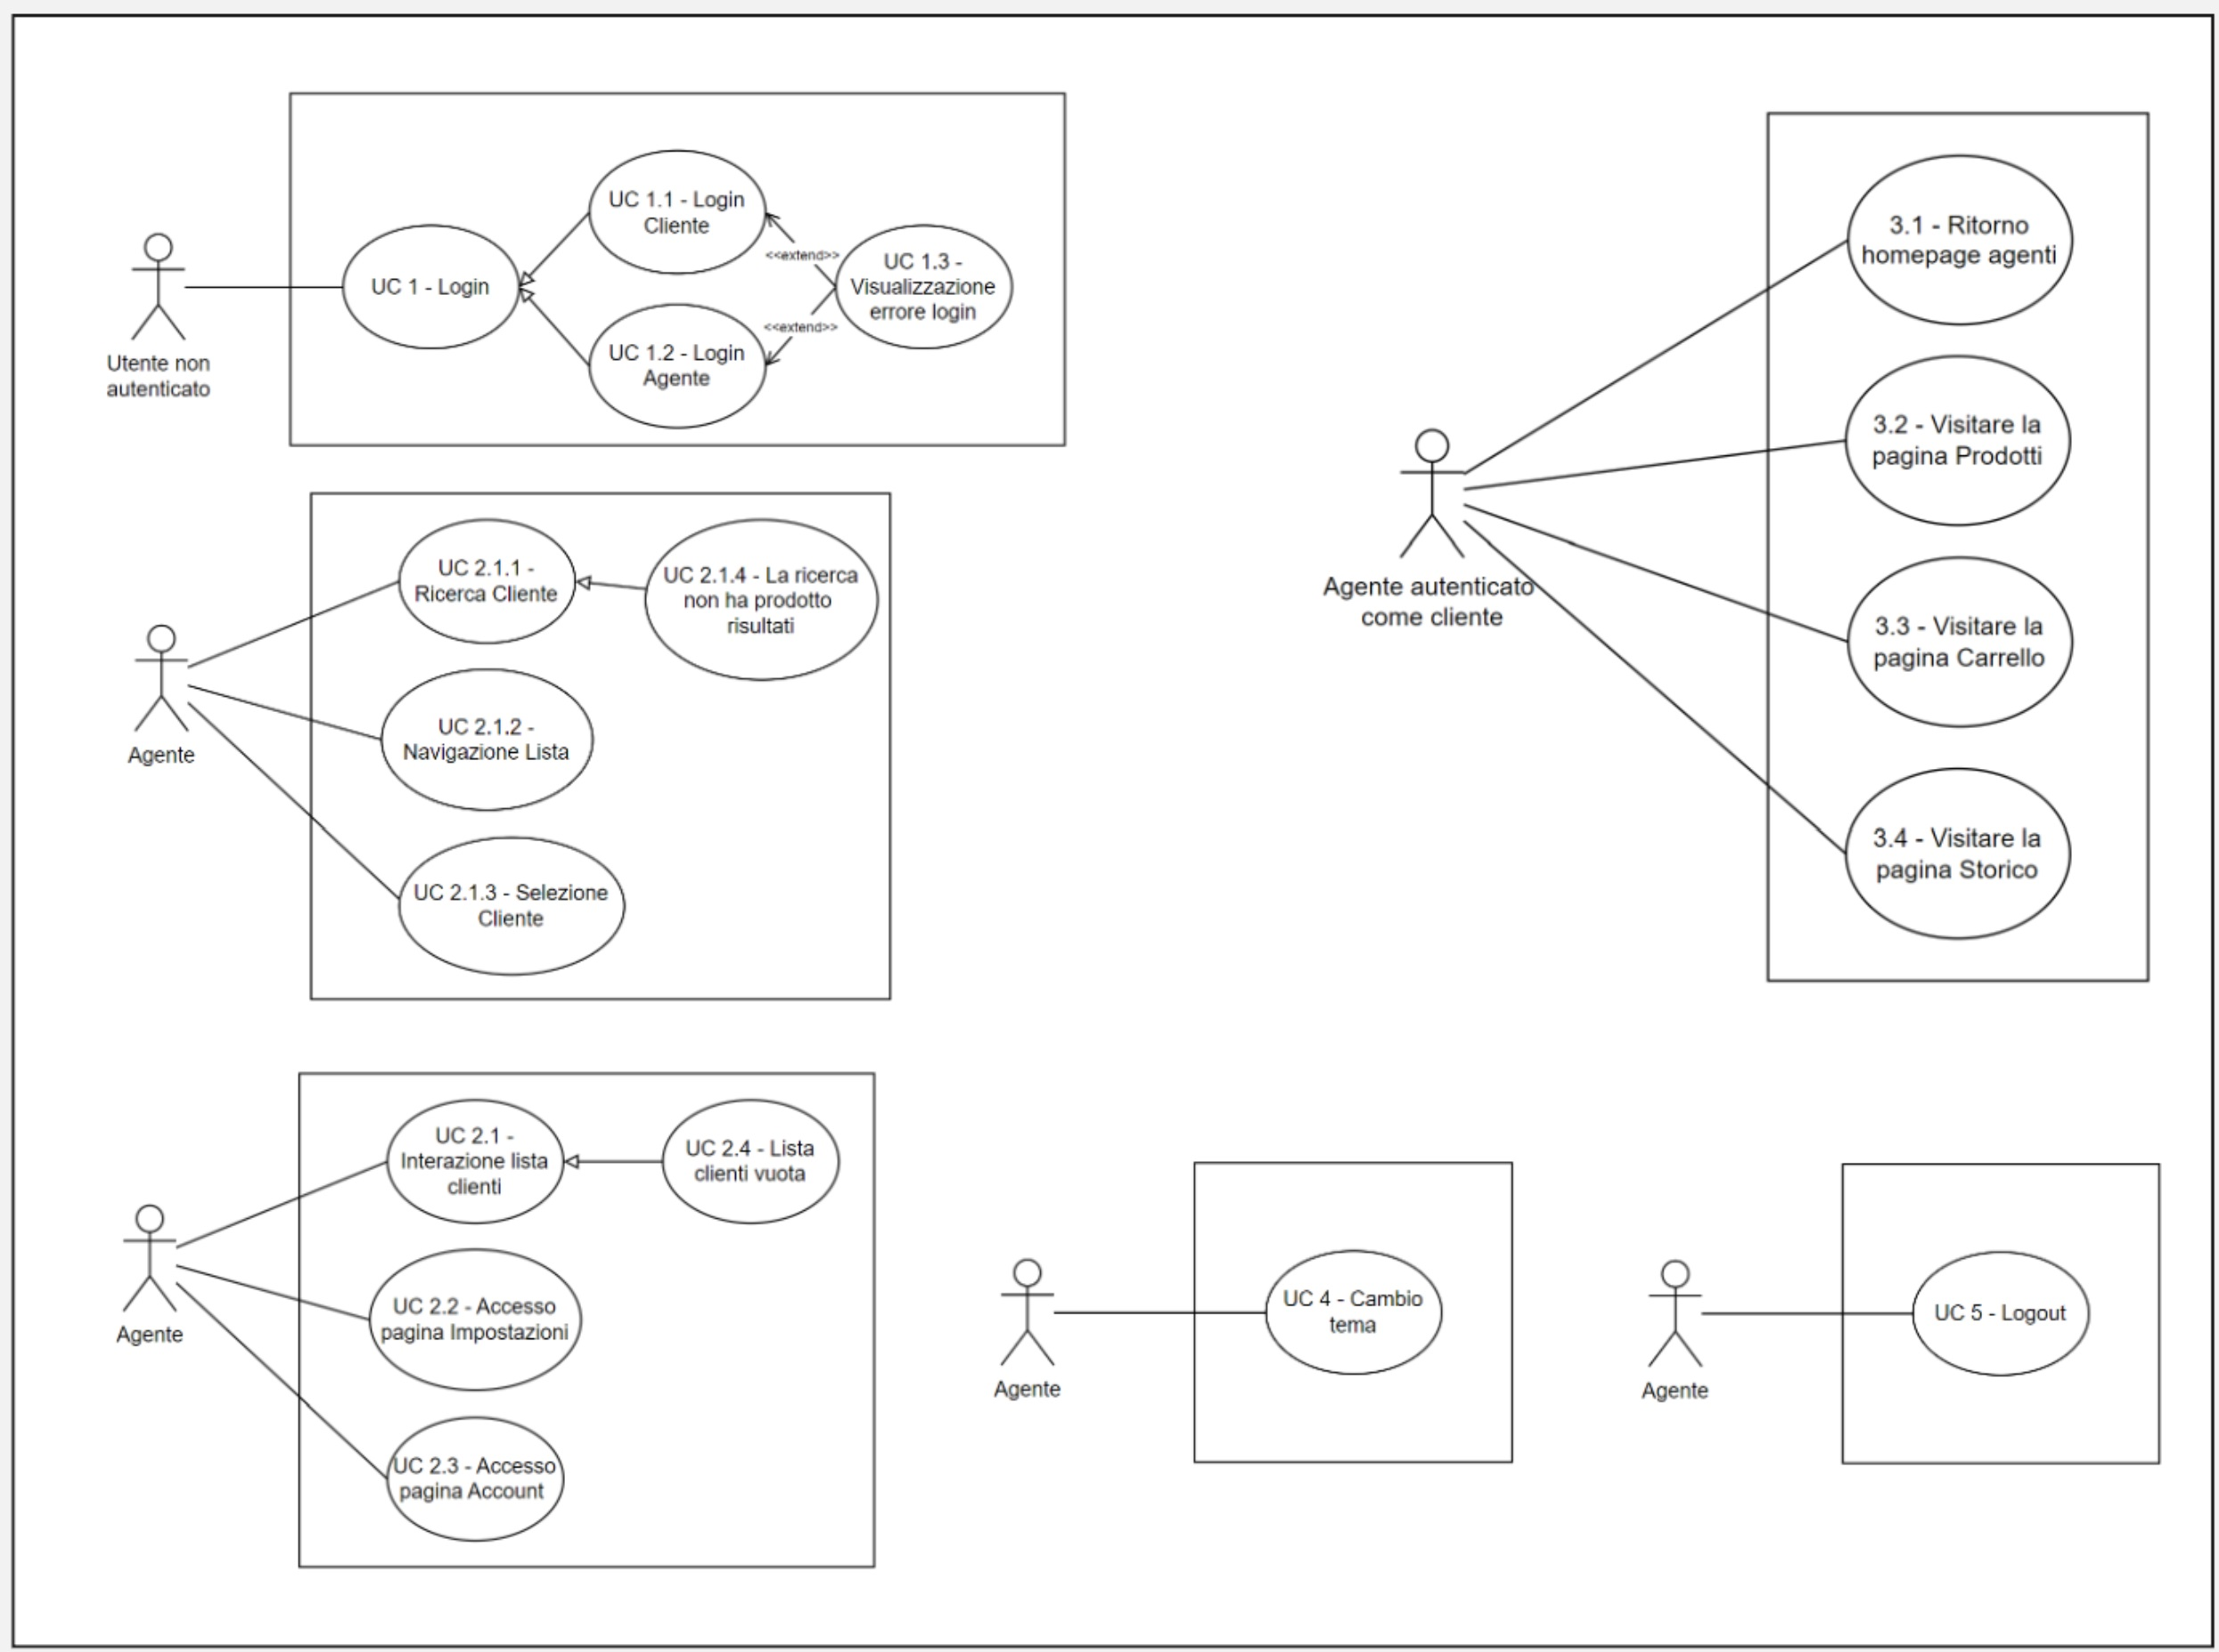
\includegraphics[width=0.7\columnwidth]{img/use_cases.jpg}
    \caption{\textit{Use Cases} modellati per il progetto}
    \label{fig:uc}
\end{figure}

Questa attività di modellazione mi ha permesso di comprendere meglio le funzionalità richieste per il 
modulo agenti e di individuare necessità implicite.\\
Nella modellazione dei casi d'uso vengono riportate diverse informazioni, come le condizioni richieste prima e dopo 
il caso d'uso, una descrizione, scenario e attori coinvolti.\\
Per comprendere i requisiti che ho riportato nel prossimo capitolo, riporto una descrizione dei tre attori principali, 
ovvero le entità (umani o altri sistemi) che interagiscono il sistema:
\begin{itemize}
    \item \textbf{Utente non autenticato}: utente che non ha completato la procedura di \textit{login}, 
          può essere un cliente o un agente;
    \item \textbf{Agente}: utente autenticato e riconosciuto dal sistema come agente aziendale;
    \item \textbf{Agente autenticato come cliente}: agente che ha selezionato un cliente e vuole operare all'interno dell'\textit{app} 
          come il cliente selezionato.
\end{itemize}

\subsection{Requisiti funzionali e non funzionali}
L'analisi dei casi d'uso permette l'identificazione e la definizione dei requisiti funzionali e non funzionali del progetto.\\
I requisiti funzionali descrivono le funzionalità specifiche che il sistema deve offrire, dettagliando il comportamento atteso 
in risposta alle diverse interazioni degli utenti. 
I requisiti non funzionali, d'altra parte, definiscono le caratteristiche qualitative del sistema, come prestazioni, 
sicurezza, usabilità e scalabilità. Sebbene non sempre esplicitamente evidenti nei casi d'uso, questi requisiti 
sono spesso impliciti nelle aspettative degli utenti. In alcuni casi le necessità che portano a descrivere questi requisiti 
non sono proprio modellabili come casi d'uso (come la necessità di fornire la documentazione sul 
progetto), pertanto la definizione dei requisiti si rivela essere un lavoro complesso quanto essenziale.\\
Il numero di requisiti soddisfatti rispetto a quelli concordati permette di avere una misura della qualità del 
lavoro svolto.\\
Ho assegnato ad ogni requisito un codice identificativo, che riporta:
\begin{itemize}
    \item \textbf{F, V, Q, U}: F rappresenta i requisiti funzionali, V i requisiti non funzionali di vincolo, Q i 
          requisiti non funzionali qualitativi e U i 
          requisiti non funzionali di usabilità;
    \item \textbf{O, D}: O per i requisiti obbligatori, D per quelli desiderabili;
    \item \textbf{id}: numero identificativo del requisito;
\end{itemize}
Per ogni requisito viene fornita anche una descrizione e la fonte da cui è tratto.
Le fonti che ho riportato nella tabella indicano da dove ho ricavato il requisito descritto, troviamo:
\begin{itemize}
    \item \textbf{UC}: il requisito descritto è stato ricavato da un caso d'uso;
    \item \textbf{Capitolato}: il requisito descritto è stato ricavato dal capitolato del progetto;
    \item \textbf{\textit{Tutor}}: il requisito descritto è stato ricavato da colloqui avuti con il \textit{tutor} aziendale 
          durante il tirocinio;
    \item \textbf{Studente}: il requisito descritto è stato ricavato da personali considerazioni sul progetto.
\end{itemize}
La tabella \ref{tab:requisiti} riporta l'elenco dei requisiti che ho individuato e che ho concordato con il \textit{tutor}:

\begin{center}
    \rowcolors{1}{}{tableGray}
    \begin{longtable}{|p{2.25cm}|p{7.75cm}|p{2.25cm}|}
    \hline
    %\rowcolor{hyperColor!5}
    \multicolumn{1}{|c|}{\textbf{Requisito}} & \multicolumn{1}{c|}{\textbf{Descrizione}} & \multicolumn{1}{c|}{\textbf{Fonte}}\\
    \hline 
    \endfirsthead
    \rowcolor{white}
    \multicolumn{3}{c}{{\bfseries \tablename\ \thetable{} -- Continuo della tabella}}\\
    \hline
    %\rowcolor{hyperColor!5}
    \multicolumn{1}{|c|}{\textbf{Requisito}} & \multicolumn{1}{c|}{\textbf{Descrizione}} & \multicolumn{1}{c|}{\textbf{Fonte}}\\
    \hline 
    \endhead
    \hline
    \rowcolor{white}
    \multicolumn{3}{|r|}{{Continua nella prossima pagina...}}\\
    \hline
    \endfoot
    \endlastfoot
    
    FO1 & Un utente deve poter effettuare il \textit{login} ed essere automaticamente riconosciuto come cliente & UC, Capitolato \\
    FO1.1 & Un cliente deve essere spostato nella \texttt{Homepage} in seguito al \textit{login} & UC, Capitolato \\
    FO1.2 & Un cliente non deve poter notare nessuna differenza rispetto alla precedente versione dell'\textit{app} & Capitolato \\
    FO2 & Un utente deve poter effettuare il \textit{login} ed essere automaticamente riconosciuto come agente & UC, Capitolato \\
    FO2.1 & Un agente deve essere spostato nella \texttt{Homepage Agenti} in seguito al \textit{login} & UC, Studente \\
    FO3 & Un utente deve visualizzare un messaggio d'errore se le credenziali sono errate & UC, Studente \\
    FO4 & Un agente deve poter visualizzare una lista con i suoi clienti & Capitolato \\
    FD4.1 & Un agente deve poter ricercare un cliente all'interno della lista dei suoi clienti & UC, \textit{Tutor} \\
    FO4.2 & Un agente deve poter navigare la lista dei suoi clienti & UC, Capitolato \\
    FO4.3 & Un agente deve poter selezionare dalla lista uno dei suoi clienti & UC, Capitolato \\
    FO4.4 & Un agente deve visualizzare un messaggio d'errore che riporta la frase "nessun cliente trovato" se la lista clienti è vuota & UC, \textit{Tutor} \\
    FD4.5 & Un agente deve visualizzare un messaggio d'errore che riporta la frase "nessun cliente trovato" se la ricerca clienti non ha prodotto risultati & UC, \textit{Tutor} \\
    FO4.6 & Un agente deve essere spostato nella pagina \texttt{Homepage} dopo aver selezionato un cliente dalla lista & UC, Studente \\
    FO4.7 & Un agente deve essere autenticato come il cliente selezionato dopo aver selezionato un cliente dalla lista & UC, Capitolato \\
    FD5 & Un agente deve poter visualizzare un menu nella \texttt{Homepage Agenti} & Studente \\
    FD5.1 & Un agente deve poter premere il pulsante "Impostazioni" dal menu nella \texttt{Homepage Agenti} & UC, Studente \\
    FD5.2 & Un agente deve essere spostato nella pagina \texttt{Impostazioni} dopo aver premuto il pulsante "Impostazioni" & UC, Studente \\
    FD5.3 & Un agente deve poter premere il pulsante "\textit{Account}" dal menu nella \texttt{Homepage Agenti} & UC, Studente \\
    FD5.4 & Un agente deve essere spostato nella pagina \texttt{Account} dopo aver premuto il pulsante "\textit{Account}" & UC, Studente \\
    FO6 & Un agente autenticato come cliente deve poter visualizzare un menu nella \texttt{Homepage} & Studente \\
    FD6.1 & Un agente autenticato come cliente deve poter ritornare alla \texttt{Homepage Agenti} premendo 
            il pulsante "\textit{Homepage} Agenti" nel menu della \texttt{Homepage} & UC, Studente \\
    FD6.2 & Un agente autenticato come cliente deve essere spostato nella pagina \texttt{Prodotti} premendo 
            il pulsante "Prodotti" nel menu della \texttt{Homepage} & UC, Capitolato \\
    FD6.2.1 & Un agente autenticato come cliente deve poter operare come il cliente selezionato nella pagina \texttt{Prodotti} & UC, Capitolato \\
    FD6.3 & Un agente autenticato come cliente deve essere spostato nella pagina \texttt{Carrello} premendo 
            il pulsante "Carrello" nel menu della \texttt{Homepage} & UC, Capitolato \\
    FD6.3.1 & Un agente autenticato come cliente deve poter operare come il cliente selezionato nella pagina \texttt{Carrello} & UC, Capitolato \\
    FD6.4 & Un agente autenticato come cliente deve essere spostato nella pagina \texttt{Storico} premendo 
            il pulsante "Storico" nel menu della \texttt{Homepage} & UC, Capitolato \\
    FD6.4.1 & Un agente autenticato come cliente deve poter operare come il cliente selezionato nella pagina \texttt{Storico} & UC, Capitolato \\
    FD7.1 & Un agente deve poter modificare il tema impostando il tema chiaro dalla pagina \texttt{Impostazioni} & UC, \textit{Tutor} \\
    FD7.2 & Un agente deve poter modificare il tema impostando il tema scuro dalla pagina \texttt{Impostazioni} & UC, \textit{Tutor} \\
    FO7.3 & Un agente non deve poter modificare la propria schermata d'avvio dalla pagina \texttt{Impostazioni} & Studente \\
    FD8 & Un agente deve poter effettuare il \textit{logout} dalla pagina \texttt{Account} & UC, \textit{Tutor} \\
    QO1 & Insieme al modulo deve essere consegnato anche un manuale tecnico & Capitolato, \textit{Tutor} \\
    QO2 & Insieme al modulo deve essere consegnato anche un manuale utente & Capitolato, \textit{Tutor} \\
    UO1 & Un agente deve visualizzare il suo nome all'interno della schermata \texttt{Homepage Agenti} & Capitolato, Studente \\
    UO2 & Un agente deve visualizzare il nome del cliente selezionato all'interno della schermata \texttt{Homepage} & Capitolato, Studente \\
    UO3 & Ogni voce della lista deve riportare alcune informazioni del cliente & \textit{Tutor} \\
    UO3.1 & Ogni voce della lista deve riportare il nome del cliente & \textit{Tutor} \\
    UO3.2 & Ogni voce della lista deve riportare l'indirizzo del cliente & \textit{Tutor} \\
    UD4 & L'applicazione deve essere disponibile nella lingua italiana & \textit{Tutor} \\
    UD5 & L'applicazione deve essere disponibile nella lingua inglese & \textit{Tutor} \\
    UD6 & Deve essere possibile ricercare un cliente nelle lista attraverso l'uso di una \textit{search bar} & \textit{Tutor} \\
    UD7 & Durante la digitazione del parametro di ricerca i risultati devono essere filtrati anche per i parametri parziali & \textit{Tutor} \\
    UD8 & Durante la ricerca i clienti devono essere filtrati secondo il parametro digitato dall'agente & \textit{Tutor} \\
    UD9 & Lo stile dell'applicazione deve essere compatibile con dispositivi \textit{tablet} & Capitolato, \textit{Tutor} \\
    VO1 & Il modulo deve utilizzare i \textit{database} di {\movi} apportando eventuali modifiche alla struttura & Capitolato, \textit{Tutor} \\
    VO2 & Il modulo deve estendere le \gls{api} esistenti sviluppate in .NET & Capitolato, \textit{Tutor} \\
    VO3 & Il modulo deve estendere le interfacce esistenti sviluppate in React Native & Capitolato, \textit{Tutor} \\
    \hline
    \hiderowcolors
    \caption{Tabella del tracciamento dei requisiti funzionali e non funzionali.}
    \label{tab:requisiti}
    \end{longtable}
\end{center}

Di seguito riporto una tabella che riepiloga i requisiti precedentemente descritti.

\begin{center}
    \rowcolors{1}{}{tableGray}
    \begin{longtable}{|>{\centering\arraybackslash}p{2.25cm}|>{\centering\arraybackslash}p{4.75cm}|>{\centering\arraybackslash}p{4.75cm}|>{\centering\arraybackslash}p{2.25cm}|}    \hline
    \multicolumn{1}{|c|}{\textbf{Tipologia}} & \multicolumn{1}{c|}{\textbf{Obbligatorio}} & \multicolumn{1}{c|}{\textbf{Desiderabile}} & \multicolumn{1}{c|}{\textbf{Totale}}\\ 
    \hline 
    \endfirsthead
    \rowcolor{white}
    \multicolumn{4}{c}{{\bfseries \tablename\ \thetable{} -- Continuo della tabella}}\\
    \hline
    \multicolumn{1}{|c|}{\textbf{Tipologia}} & \multicolumn{1}{c|}{\textbf{Obbligatorio}} & \multicolumn{1}{c|}{\textbf{Desiderabile}} & \multicolumn{1}{c|}{\textbf{Totale}}\\ \hline 
    \endhead
    \hline
    \rowcolor{white}
    \multicolumn{4}{|r|}{{Continua nella prossima pagina...}}\\
    \hline
    \endfoot
    \endlastfoot 

    % Insert your table rows here
    \textbf{Funzionale} & 13 & 17 & 30 \\
    \textbf{Di vincolo} & 3 & 0 & 3 \\
    \textbf{Qualitativi} & 2 & 0 & 2 \\
    \textbf{Usabilità} & 5 & 6 & 11 \\
    \textbf{Totale} & 23 & 23 & 46 \\

    \hline
    \hiderowcolors
    \caption{Riepilogo requisti}
    \label{tab:requisiti riassuntos}
    \end{longtable}
\end{center}





